% 卒業研究前刷テンプレート
% lualatex用

\RequirePackage{plautopatch}

\documentclass[a4paper,10pt]{ltjsarticle}
\usepackage{luatexja}
\usepackage{enumitem} % リストカスタマイズ用
\usepackage{geometry}
\usepackage{multicol}
\usepackage{amsmath}
\usepackage{titlesec}
\usepackage{flushend}
\usepackage{graphicx}
\usepackage{here}

\geometry{
top=20mm,
bottom=20mm,
left=20mm,
right=20mm
}
\setlength{\columnsep}{7.5mm}

\setlength{\baselineskip}{14pt}
\setlength{\parindent}{1\zw}

\titleformat{\section}{\large\bfseries}{\thesection}{1\zw}{}
\titlespacing{\section}{0pt}{*1}{*1}
\titleformat{\subsection}{\large\bfseries}{\thesubsection}{1\zw}{}
\titlespacing{\subsection}{0pt}{*1}{*1}
\titleformat{\subsubsection}{\large\bfseries}{\thesubsubsection}{1\zw}{}
\titlespacing{\subsubsection}{0pt}{*1}{*1}

\pagestyle{empty}

\SetLabelAlign{parright}{\parbox[t]{\labelwidth}{\raggedleft#1}}

\makeatletter
\def\@maketitle{
\begin{flushright}
{\large \@date}
\end{flushright}
\begin{center}
{\LARGE \@title \par}
\end{center}
\begin{flushright}
{\large \@author}
\end{flushright}
\par\vskip 1.5em
}
\makeatother

\title{\huge ドローンにおける直線中継伝送のアクセス制御方式の検討評価\\
\Large Study and Evaluation of Access Control Schemes for Rectilinear Relay transmission in drones
}

\author{
T5-25 \:中村 優\\
指導教員 \: 設樂 勇
}

\date{}

\begin{document}
% タイトル部分は1カラムで表示
\twocolumn[
\maketitle
]

% ---------
% 本文開始
% ---------
\section{はじめに}
ドローンを用いたネットワークにおいて,オーバーリーチの問題を解決するために送信信号の届く中継局まで一度に中継する CTR(Cooperation Through Relay)方式[1]が提案されている. 本稿では,提案手法において干渉/誤りが生じた際のスループット特性を従来方式と比較し評価する.
\section{従来方式の概要}
図1に従来方式の概要を示す.従来の中継伝送では 1 ホップずつ中継するが,自由空間では,伝搬損失が少ないため送信信号が中継先のドローン(図1\#3)より遠くのドローン(図1\#4)に到達し干渉が生じる.そのため,従来方式は,オーバーリーチ干渉によってチャネル利用効率が低下する.また,従来方式で干渉が生じ,再送を行う際には,フォールバック制御により伝送レートを下げることでSNR(Signal to Noise Ratio)が低くてもパケットを受信できるようにしているが,伝送レートの低下に伴って送信時間や再送によるオーバヘッドが増加してしまう課題がある.


\begin{figure}[htbp]
  \centering
  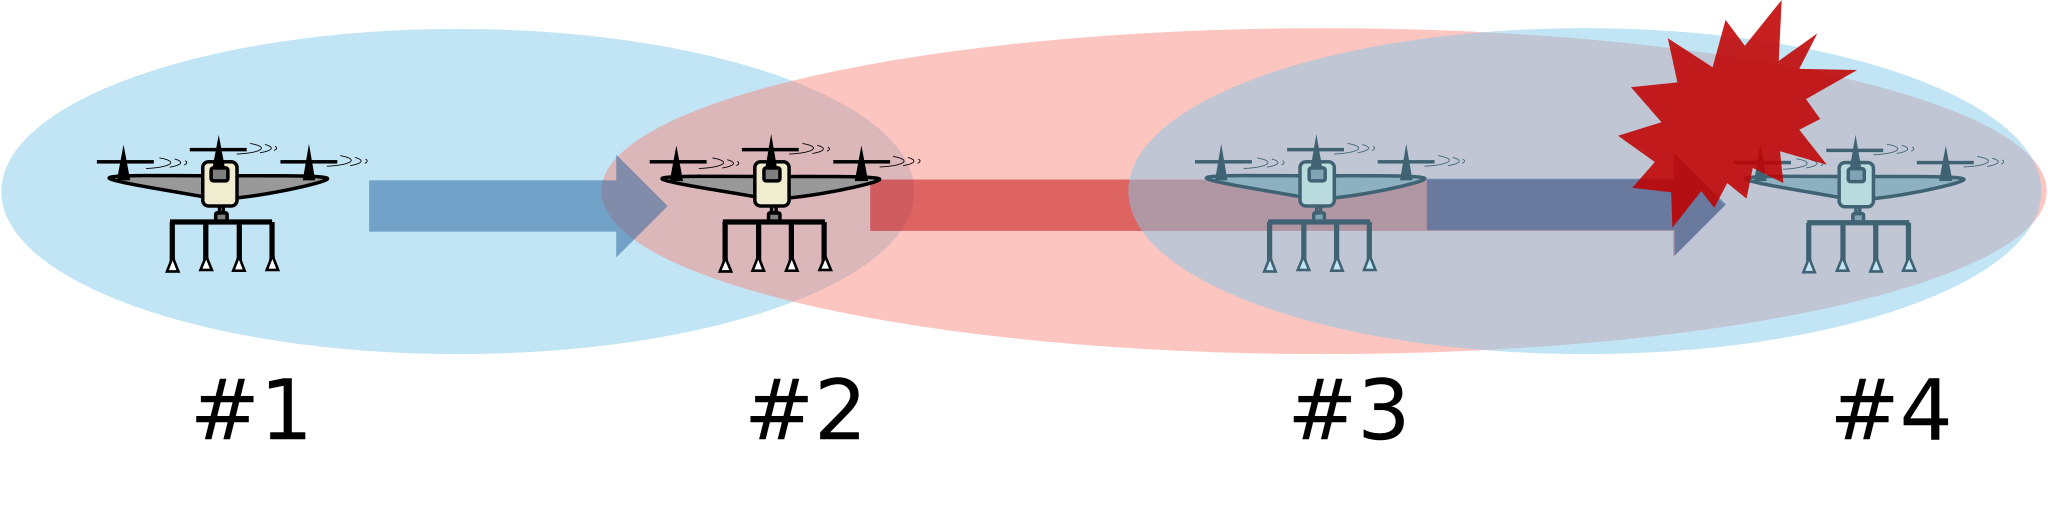
\includegraphics[width=\linewidth]{cenventional_topology.png} % 図のファイル名を指定
  \caption{従来の方式の概要}
  \label{fig:従来の方式のトポロジー} % 参照用ラベル
\end{figure}

\section{CTR方式の概要}
\subsection{CTR方式のアクセス制御}
図2に示すCTR方式は,送信信号の届く範囲の最終中継局(図 1\#4)まで一度に信号を送信し,通信経路の中継局(図 1\#3)もパケットを受信する.最終中継局がパケットの受信に失敗した場合は,直線経路の中継局\#3が\#4 の代わりに次の中継局にパケットを中継する.そのためオーバーリーチ干渉の影響を減らすとともに中継ホップ数も減るので中継オーバヘッドも削減することができる.
\begin{figure}[htbp]
  \centering
  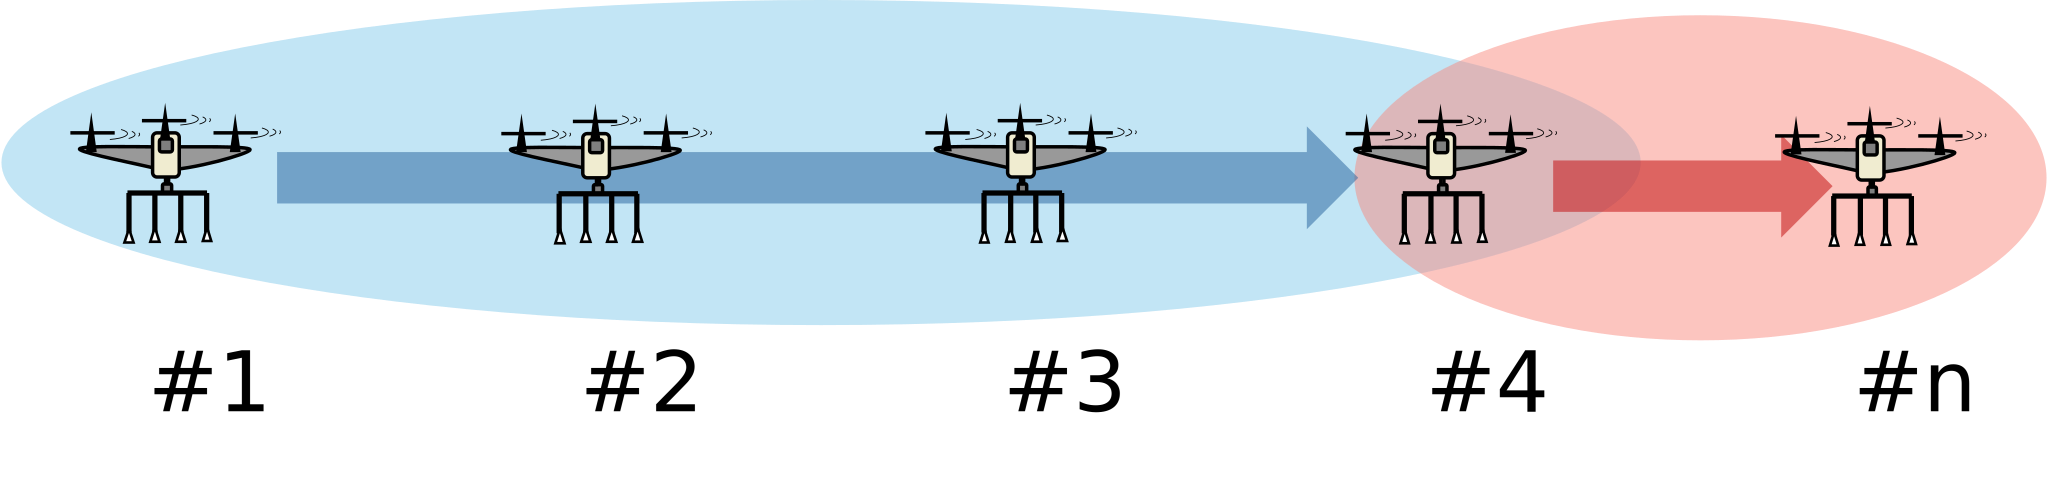
\includegraphics[width=\linewidth]{CTR_topology.png} % 図のファイル名を指定
  \caption{CTR方式の概要}
  \label{fig:CTR方式のトポロジー} % 参照用ラベル
\end{figure}
\\ 図3にCTR方式の詳細なアクセス制御手順を示す.送信局はACK(Acknowledgement)のduration時間が記述されたパケットを送信し,パケットを受信した中継局は送信局に対して ACK duration 時間後にACKを返信する.このとき,ACKを受信した直線経路上の中継局はACKの送信待ちをキャンセルする.最終中継局(図2\#4)がパケット を受信できない場合は\#3が送信局の\#1に ACKを送信し,\#4の代わりに中継する.
ACK duration はスロットタイム区切りとなっており,最終受信中継局が最もACK duration が短く,送信局に近づくにつれて1 ずつスロットタイム増加していく.
したがって,このCTR 方式は信号が届く最大の範囲を推定する必要がある.そのため,送信電力の制御に加え各端末
のSNRの受信電力閾値から自律的に判断し中継制御を行う.
\begin{figure}[H]
  \centering
  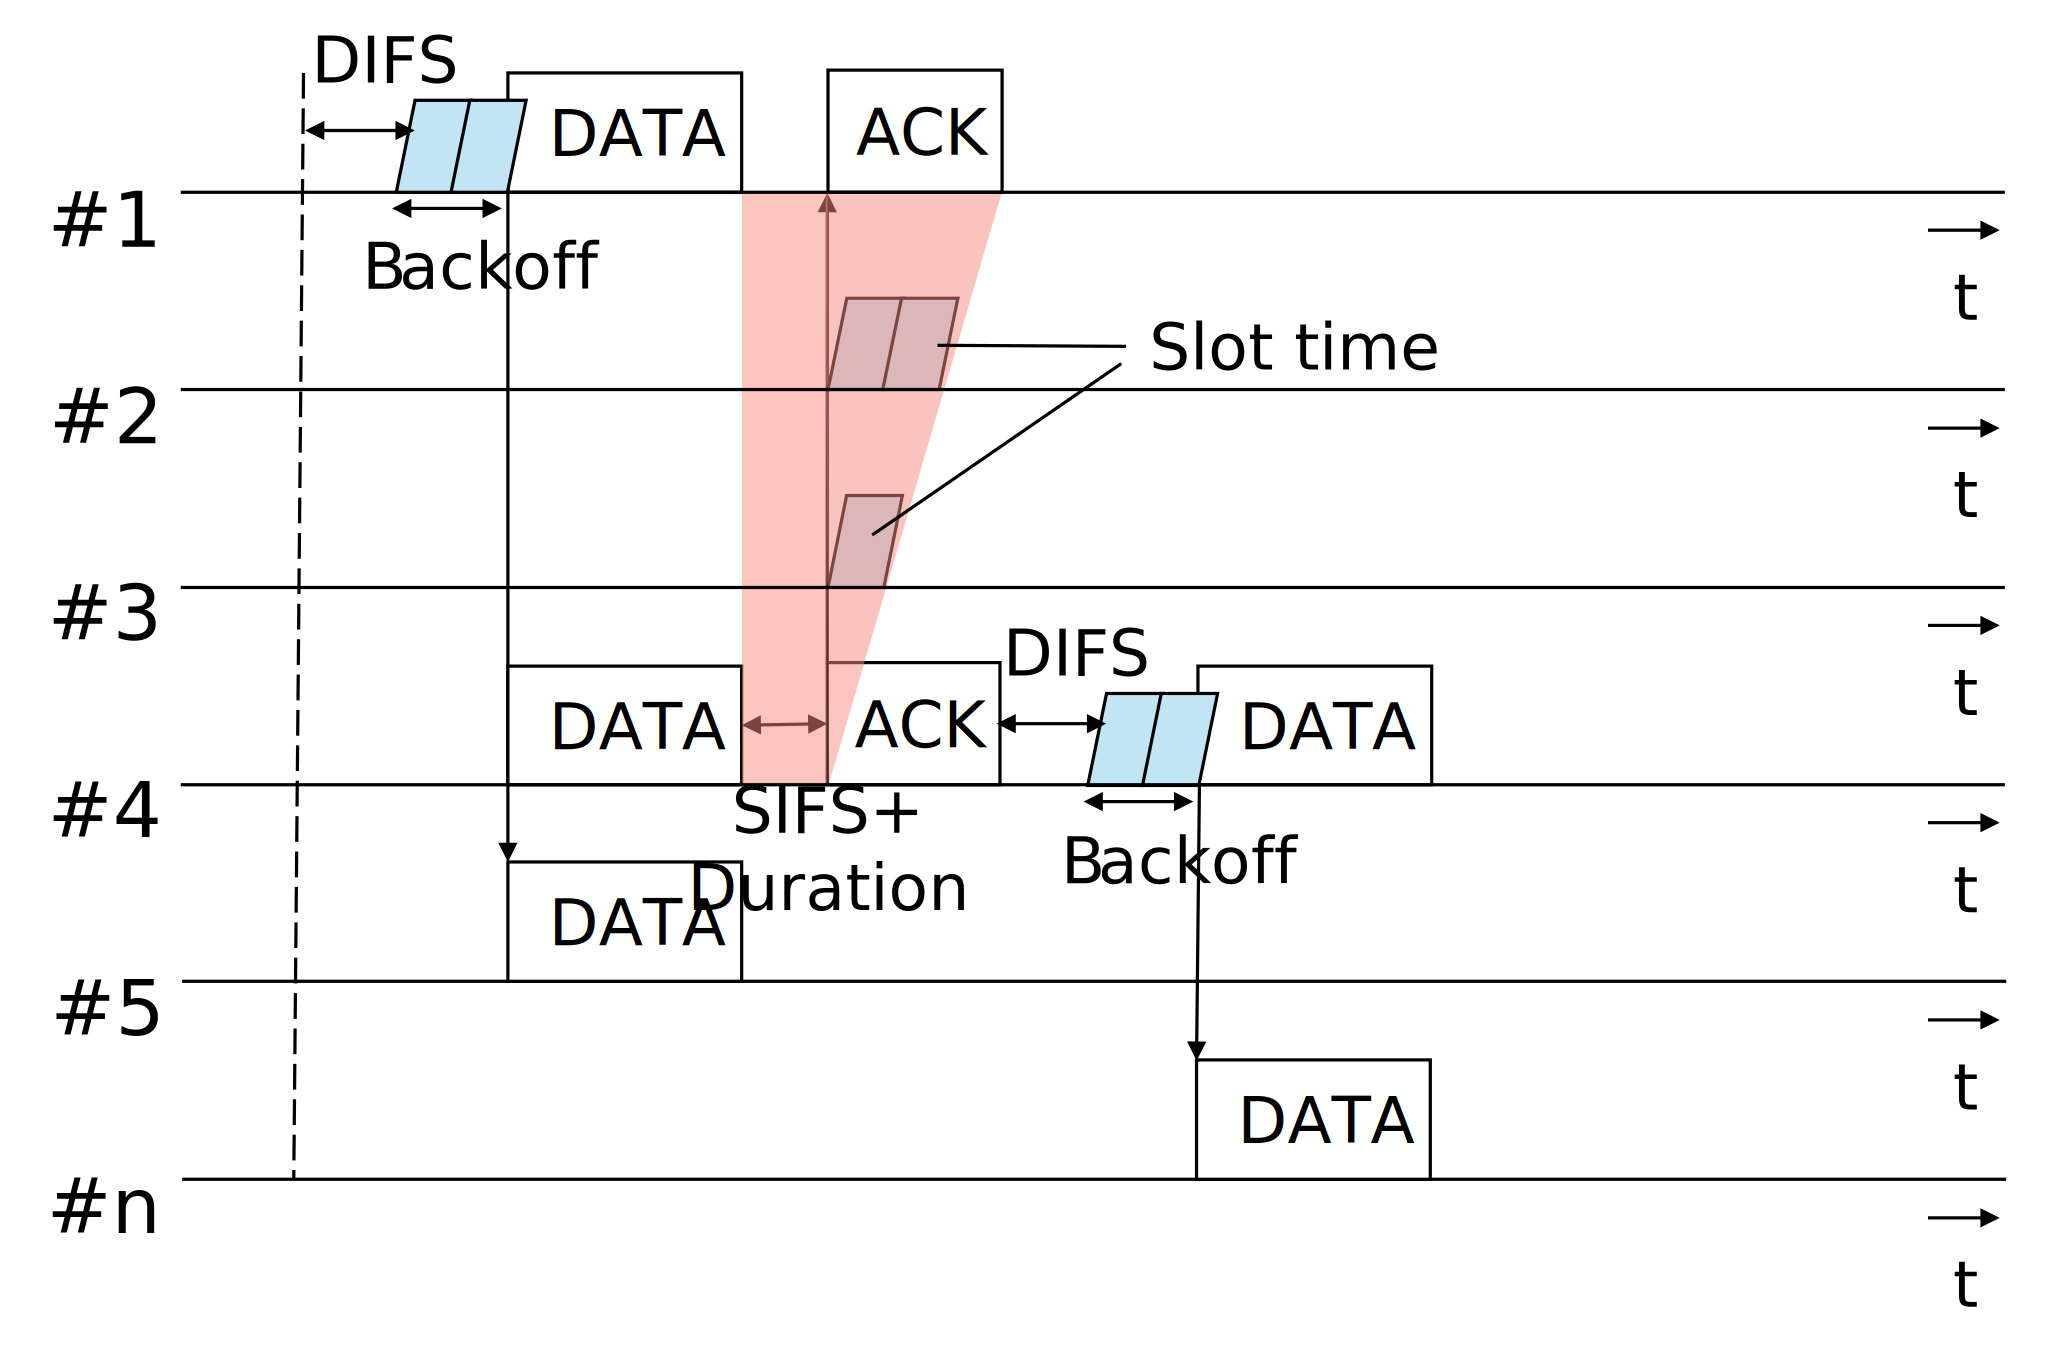
\includegraphics[width=\linewidth]{CTR_accsess.png} % 図のファイル名を指定
  \caption{CTR方式のアクセス制御}
  \label{fig:CTR方式のアクセス制御} % 参照用ラベル
\end{figure}
\subsection{CTR方式の効果}
CTR 方式の特徴である中継局をスルーすることによる効果を確認する.
中継の総伝送距離は1000mとし,50m間隔で直線状に20台のドローンを配置した.アンテナの送受信利得は0dBi,送信電力は10dBmとした.周波数は 2.4GHz,伝送レートはIEEE 802.11gを参考にし,伝搬損失は自由空間伝搬損失とした.
評価内容は従来の1 ホップ中継(65 Mbps) と中継局を1 台スルー(39 Mbps) した場合,
および中継局を3 台スルー(19.5 Mbps) した場合におけるスループット特性を確認する.括弧内は使用可能な伝送レートである.
干渉/誤りは無いとする.
\begin{figure}[H]
  \centering
  \includegraphics[width=\linewidth]{throughtput_vs_placement_50m_max_distance_3.png} % 図のファイル名を指定
  \caption{ドローンをスルーした時のスループット}
  \label{fig:Throughput_through} % 参照用ラベル
\end{figure}
\section{比較結果}
本稿では,CTR方式において誤りが生じる条件にて評価を行う.従来方式では再送時のフォールバック制御により伝送レートを一つ下の12Mbpsとする.中継局を3台スルーした場合におけるスループット特性を評価した.このときパケット誤り率を3%と20%とし,1000回試行したときの従来の方式とCTR方式の平均のスループット特性を比較した.
この結果からいずれの条件でもCTR方式が従来方式よりも高いスループットが得られることを確認した.また, 誤り率3%と20%を比較すると20%の方が従来方式よりスループットが高くなることから, 従来方式よりもCTR方式は誤り率が高い条件においても高速に中継伝送が可能なことを確認した.

\begin{figure}[H]
  \centering
  \includegraphics[width=\linewidth]{throughput_probabilistic_retry_0.03.png} % 図のファイル名を指定
  \caption{誤り率3\%の時のスループット}
  \label{fig:Throughput_0.03} % 参照用ラベル
\end{figure}
\begin{figure}[H]
  \centering
  \includegraphics[width=\linewidth]{throughput_probabilistic_retry_0.2.png} % 図のファイル名を指定
  \caption{誤り率20\%の時のスループット}
  \label{fig:Throughput_0.2} % 参照用ラベル
\end{figure}
\section{まとめ}
本研究では直線に配置されたドローン中継伝送におけるオー
バリーチ干渉の影響を計算機シミュレーションなどで確認し,
干渉問題を解決するために送信信号の届く中継局まで一回で中
継するCTR 方式を提案した.また,初期検討としてCTR 方
式の中継局をスルーすることによる効果を確認した.評価結
果から従来の1 ホップ中継と比較してCTR 方式は高いスルー
プットが得られることを確認した.今後は,干渉や誤りを含め
た評価を行い,より詳細に提案方式を評価する予定である.
\\参考文献
\\1. [1]設樂,他,“ドローンの直線中継伝送におけるアクセ
ス制御方式の一検討,” 電子情報通信学会大会講演
論文 B‐11‐2,2018 年 9 月
% ---------
% 文献リスト
% ---------
\bibliography{arxiv} % bibファイルを指定 (例: arxiv.bib)
\bibliographystyle{junsrt}

\end{document}
